\subsubsection{Renderer}
\label{sec:renderer}
\hspace{\parindent} The renderer uses \hyperref[context]{\ref*{context} Context} that provides global properties of this renderer.\\
Despite the fact that the \hyperref[sec:headset]{\ref*{sec:headset} Headset} is not responsible for the \hyperref[sec:rendering_process]{\ref*{sec:rendering_process} Rendering Process}, that class has a big influence on the renderer. As our engine is designed for virtual reality purposes, we decided that headset's swapchain has a priority over window's swapchain due to the fact that rendering depends on the image created by the headset (for an instance from the user experience it can be noticed by not having anything displayed on the window if a headset stays in standby mode). Therefore, \texttt{Headset} class is explained here instead of having separated dedicated section.

Graphical presentation of the relations in the renderer is portrayed in the following image.
The same applies to \texttt{MirroView} class that is used as an intermediate layer of abstraction between \hyperref[window]{\ref*{window} \texttt{Window} class}, and the renderer.
\label{fig:renderer}
\begin{figure}[H]
  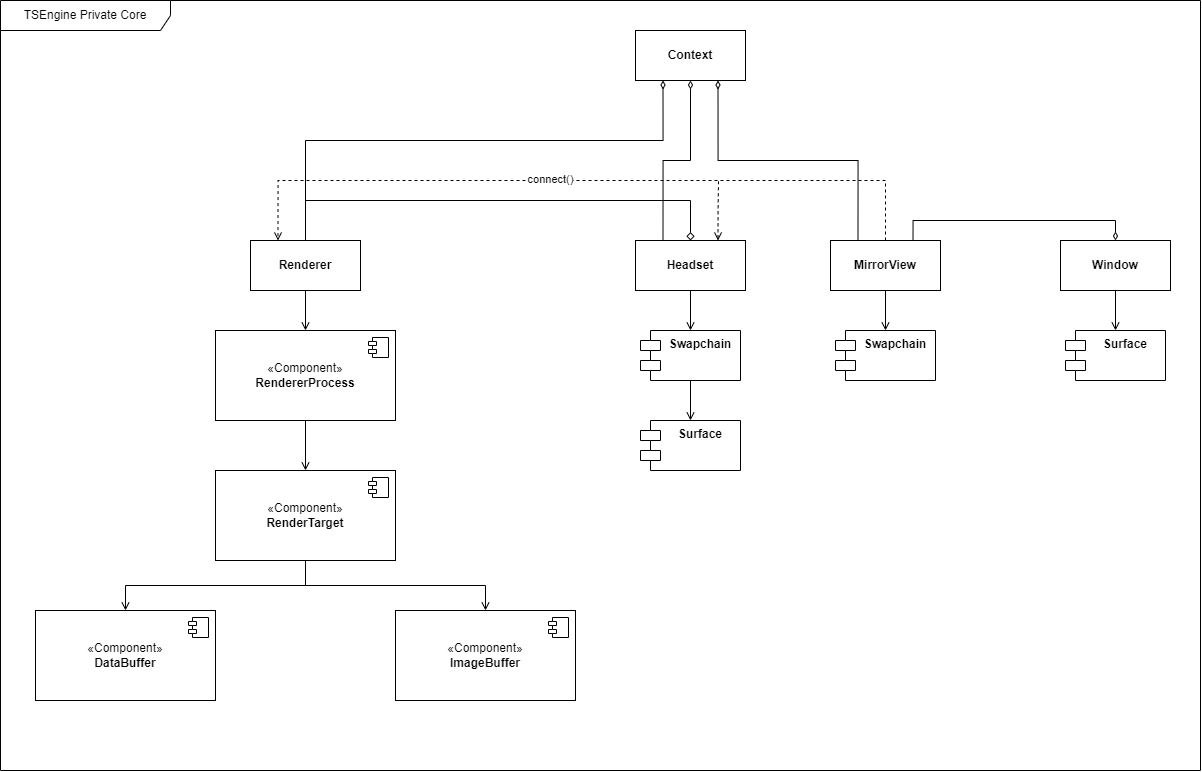
\includegraphics[width=\linewidth]{renderer.png}
  \caption{Renderer relations}
\end{figure}
\newpage
We can distinguish the front-end of the renderer being the part of ECS - \hyperref[sec:renderer_system]{\ref*{sec:renderer_system}. ECS Renderer System}, but also back-end in classes:
\begin{itemize}
    \item \texttt{Renderer}\\
    Comprehensive component of the engine core that manages various aspects of the rendering pipeline in a Vulkan environment that plays a role of back-end of the renderer. It orchestrates render processes, manages Vulkan resources like command pools and descriptor pools, and handles different pipelines for rendering. The class's structure emphasizes controlled resource management, synchronization, and the ability to handle multiple frames in flight.
\begin{lstlisting}[language=c++, caption=\texttt{Renderer} class (./engine/src/core/renderer.h)]
class Renderer
{
    TS_NOT_COPYABLE_AND_MOVEABLE(Renderer);

    static constexpr size_t framesInFlightCount{2};

public:
    Renderer(const Context& ctx, const Headset& headset);

    virtual ~Renderer();

    void createRenderer();
    void render(const size_t swapchainImageIndex);
    void submit(const bool useSemaphores) const;

    [[nodiscard]] VkSemaphore getCurrentDrawableSemaphore() const;
    [[nodiscard]] VkSemaphore getCurrentPresentableSemaphore() const;
    [[nodiscard]] VkCommandBuffer getCurrentCommandBuffer() const;

private:
    void createVertexIndexBuffer();
    void updateUniformData(const std::unique_ptr<RenderProcess>& renderProcess);
    void initRendererFrontend();

    const Context& mCtx;
    const Headset& mHeadset;
    VkCommandPool mCommandPool{};
    VkDescriptorPool mDescriptorPool{};
    VkDescriptorSetLayout mDescriptorSetLayout{};
    VkPipelineLayout mPipelineLayout{};
    std::array<std::unique_ptr<RenderProcess>, framesInFlightCount> mRenderProcesses{};
    std::shared_ptr<Pipeline> mGridPipeline, mNormalLightingPipeline, mPbrPipeline, mLightCubePipeline;
    size_t mIndexOffset{};
    std::unique_ptr<DataBuffer> mVertexIndexBuffer;
    size_t mCurrentRenderProcessIndex{};
};
\end{lstlisting}
    \item Renderer components:
    \begin{itemize}
    \item \texttt{DataBuffer}\\
    It encapsulates Vulkan buffer handling, abstracting details such as buffer creation, memory management, and data transfer between RAM and GPU's memory.
\begin{lstlisting}[language=c++, caption=\texttt{DataBuffer} class (./engine/src/core/data\_buffer.h)]
class DataBuffer final
{
    TS_NOT_COPYABLE_AND_MOVEABLE(DataBuffer);

public:
    DataBuffer(const Context& ctx);
    ~DataBuffer();

    void createDataBuffer(const VkBufferUsageFlags bufferUsageFlags, const VkMemoryPropertyFlags memoryProperties, const VkDeviceSize size);

    [[nodiscard]] VkBuffer getBuffer() const { return mBuffer; }

    void copyTo(const DataBuffer& target, VkCommandBuffer commandBuffer, VkQueue queue) const;
    void* map() const;
    void unmap() const;

private:
    const Context& mCtx;
    VkBuffer mBuffer{};
    VkDeviceMemory mDeviceMemory{};
    VkDeviceSize mSize{};
};
\end{lstlisting}
    \item \texttt{ImageBuffer}\\
    It is designed for encapsulation of the creation and management of Vulkan images, device memory allocations, and image views.
\begin{lstlisting}[language=c++, caption=\texttt{ImageBuffer} class (./engine/src/core/image\_buffer.h)]
class ImageBuffer final
{
    TS_NOT_COPYABLE_AND_MOVEABLE(ImageBuffer);

public:
    ImageBuffer(const Context& ctx) : mCtx{ctx}
    {}
    ~ImageBuffer();

    void createImage(
        VkExtent2D size,
        VkFormat format,
        VkImageUsageFlagBits usage,
        VkSampleCountFlagBits samples,
        VkImageAspectFlags aspect,
        size_t layerCount);

    [[nodiscard]] VkImageView getVkImageView() const { return mImageView; }

private:
    const Context& mCtx;
    VkImage mImage{};
    VkDeviceMemory mDeviceMemory{};
    VkImageView mImageView{};
};
\end{lstlisting}
    \item \texttt{Pipeline}\\
    This class encompasses the complexity of Vulkan's many different stages and settings, from shader stages to fixed-function state like blending, depth testing, providing a more streamlined interface for setting up and using these pipelines in rendering operations.
\begin{lstlisting}[language=c++, caption=\texttt{Pipeline} class (./engine/src/core/pipeline.h)]
class Pipeline final
{
    TS_NOT_COPYABLE_AND_MOVEABLE(Pipeline);

public:
    Pipeline(const Context& ctx);
    ~Pipeline();

    void createPipeline(
        VkPipelineLayout pipelinelineLayout,
        VkRenderPass renderPass,
        const std::string& vertexFilename,
        const std::string& fragmentFilename,
        const std::vector<VkVertexInputBindingDescription>& vertexInputBindingDescriptions = {},
        const std::vector<VkVertexInputAttributeDescription>& vertexInputAttributeDescriptions = {});

    void bind(const VkCommandBuffer commandBuffer) const;

private:
    const Context& mCtx;
    VkPipeline mPipeline{};
};
\end{lstlisting}
    \item \texttt{RenderTarget}\\
    It is designed to encapsulate the concept of a render target in Vulkan. It manages the creation and lifecycle of a framebuffer and associated image views, which are fundamental to rendering operations. The framebuffer combines color and depth and stencil attachments, which are used during a render pass.
\begin{lstlisting}[language=c++, caption=\texttt{RenderTarget} class (./engine/src/core/render\_target.h)]
class RenderTarget final
{
    TS_NOT_COPYABLE_AND_MOVEABLE(RenderTarget);

public:
    RenderTarget(VkDevice device, VkImage image) : mDevice(device), mImage(image)
    {}
    ~RenderTarget();

    void createRenderTarget(
        VkImageView colorImageView,
        VkImageView depthImageView,
        VkExtent2D size,
        VkFormat format,
        VkRenderPass renderPass,
        uint32_t layerCount);

    [[nodiscard]] VkImage getImage() const { return mImage; }
    [[nodiscard]] VkFramebuffer getFramebuffer() const { return mFramebuffer; };

private:
    VkDevice mDevice{};
    VkImage mImage{};
    VkImageView mImageView{};
    VkFramebuffer mFramebuffer{};
};
\end{lstlisting}
    \item \texttt{RendererProcess}
    It manages uniform data for objects and lights, handles synchronization primitives, and maintains various Vulkan objects essential for rendering operations.
\begin{lstlisting}[language=c++, caption=\texttt{RendererProcess} class (./engine/src/core/renderer\_process.h)]
class RenderProcess final
{
    TS_NOT_COPYABLE_AND_MOVEABLE(RenderProcess);

public:
    RenderProcess(const Context& ctx, const Headset& headset);
    ~RenderProcess();

    void createRendererProcess(
        const VkCommandPool commandPool,
        const VkDescriptorPool descriptorPool,
        const VkDescriptorSetLayout descriptorSetLayout,
        const size_t modelsNum,
        const size_t lightsNum);

    struct IndivialData final
    {
        math::Mat4 model;
    };
    std::vector<IndivialData> mIndividualUniformData{};
    
    struct LightData final
    {
        std::array<math::Vec3, LIGHTS_N> positions;
    } mLightsUniformData{};

    struct CommonUniformData final
    {
        math::Vec3 cameraPosition;
        std::array<math::Mat4, 2> viewMats;
        std::array<math::Mat4, 2> projMats;
    } mCommonUniformData{};

    void updateUniformBufferData();

    [[nodiscard]] VkCommandBuffer getCommandBuffer() const { return mCommandBuffer; }
    [[nodiscard]] VkFence getFence() const { return mFence; }
    [[nodiscard]] VkDescriptorSet getDescriptorSet() const { return mDescriptorSet; }
    [[nodiscard]] VkSemaphore getDrawableSemaphore() const { return mDrawableSemaphore; }
    [[nodiscard]] VkSemaphore getPresentableSemaphore() const { return mPresentableSemaphore; }

private:
    const Context& mCtx;
    VkCommandBuffer mCommandBuffer{};
    VkSemaphore mDrawableSemaphore{}, mPresentableSemaphore{};
    VkFence mFence{};
    std::unique_ptr<DataBuffer> mUniformBuffer;
    void* mUniformBufferMemory{};
    VkDescriptorSet mDescriptorSet{};
    const Headset& mHeadset;
};
\end{lstlisting}
    \end{itemize}
    \item Renderer-related:
    \begin{itemize}
        \item \texttt{Headset}\\
        \label{sec:headset}
        \texttt{Headset} tracks the state of the device and its swapchain.
\begin{lstlisting}[language=c++, caption=\texttt{Headset} class (./engine/src/core/headset.h)]
class Headset final
{
    TS_NOT_COPYABLE_AND_MOVEABLE(Headset);

    static constexpr XrReferenceSpaceType spaceType{XR_REFERENCE_SPACE_TYPE_STAGE};
    static constexpr VkFormat colorFormat{VK_FORMAT_R8G8B8A8_SRGB};
    static constexpr VkFormat depthFormat{VK_FORMAT_D32_SFLOAT};

public:
    Headset(const Context& ctx);
    ~Headset();

    enum class BeginFrameResult
    {
        RENDER_FULLY,
        RENDER_SKIP_PARTIALLY,
        RENDER_SKIP_FULLY
    };

    void init();

    BeginFrameResult beginFrame(uint32_t& swapchainImageIndex);

    void createVkRenderPass();
    void createXrSession();
    void createXrSpace();
    void createXrSwapchain();
    void endFrame(bool skipReleaseSwapchainImage) const;

    [[nodiscard]] XrSession getXrSession() const { return mXrSession; }
    [[nodiscard]] VkRenderPass getVkRenderPass() const { return mVkRenderPass; }
    [[nodiscard]] bool isExitRequested() const { return mIsExitRequested; }
    [[nodiscard]] XrSpace getXrSpace() const { return mXrSpace; }
    [[nodiscard]] XrFrameState getXrFrameState() const { return mXrFrameState; }
    [[nodiscard]] std::shared_ptr<RenderTarget> getRenderTarget(size_t swapchainImageIndex) const { return mSwapchainRenderTargets.at(swapchainImageIndex); }
    [[nodiscard]] VkExtent2D getEyeResolution(int32_t eyeIndex) const;
    [[nodiscard]] size_t getEyeCount() const { return mEyeCount; }
    [[nodiscard]] math::Mat4 getEyeViewMatrix(size_t eyeIndex) const { return mEyeviewMats.at(eyeIndex); }
    [[nodiscard]] math::Mat4 getEyeProjectionMatrix(size_t eyeIndex) const { return mEyeProjectionMatrices.at(eyeIndex); }

private:
    void createViews();
    void beginSession() const;
    void endSession() const;

    const Context& mCtx;
    VkRenderPass mVkRenderPass{};
    XrSession mXrSession{};
    XrSpace mXrSpace{};
    uint32_t mEyeCount{};
    std::vector<XrViewConfigurationView> mEyeViewInfos;
    std::vector<XrView> mEyePoses;
    std::unique_ptr<ImageBuffer> mColorBuffer;
    std::unique_ptr<ImageBuffer> mDepthBuffer;
    XrSwapchain mXrSwapchain{};
    std::vector<std::shared_ptr<RenderTarget>> mSwapchainRenderTargets;
    std::vector<XrCompositionLayerProjectionView> mEyeRenderInfos;
    std::vector<math::Mat4> mEyeviewMats;
    std::vector<math::Mat4> mEyeProjectionMatrices;
    bool mIsExitRequested{};
    XrFrameState mXrFrameState{};
    XrSessionState mXrSessionState{};
    XrViewState mXrViewState{};
};
\end{lstlisting}
        \item \texttt{MirrorView}\\
        \texttt{MirrorView} presents framebuffer on the connected a window's surface.
\begin{lstlisting}[language=c++, caption=\texttt{MirrorView} class (./engine/src/core/mirror\_view.h)]
class MirrorView final
{
    TS_NOT_COPYABLE_AND_MOVEABLE(MirrorView);

    static constexpr VkFormat colorFormat{VK_FORMAT_B8G8R8A8_SRGB};
    static constexpr VkPresentModeKHR presentMode{VK_PRESENT_MODE_FIFO_KHR};
    static constexpr size_t mirrorEyeIndex{1};

public:
    MirrorView(const Context& ctx, const std::shared_ptr<Window> window);
    ~MirrorView();

    enum class RenderResult
    {
        VISIBLE,
        INVISIBLE
    };

    void createSurface();
    void connect(const Headset* headset, const Renderer* renderer);
    MirrorView::RenderResult render(uint32_t swapchainImageIndex);
    void present();

    void onWindowResize() { mIsResizeDetected = true; }

    [[nodiscard]] VkSurfaceKHR getSurface() const { return mSurface; }

private:
    void recreateXrSwapchain();
    void getSurfaceCapabilitiesAndExtent();
    bool isWindowMinimize();
    void pickSurfaceFormat();
    void createSwapchain();

    const Context& mCtx;
    const std::weak_ptr<Window> mWindow;
    const Headset* mHeadset;
    VkSurfaceKHR mSurface{};
    const Renderer* mRenderer;
    VkSurfaceCapabilitiesKHR mSurfaceCapabilities{};
    VkSwapchainKHR mSwapchain{};
    VkExtent2D mSwapchainResolution{};
    std::vector<VkImage> mSwapchainImages;
    VkSurfaceFormatKHR mSurfaceFormat{};
    bool mIsResizeDetected{};
    uint32_t mDestinationImageIndex{};
};
\end{lstlisting}
    \end{itemize}
\end{itemize}